\documentclass[border=5mm,tikz]{standalone}
\usepackage{tikz-cd}
\usepackage{amsmath}

\begin{document}

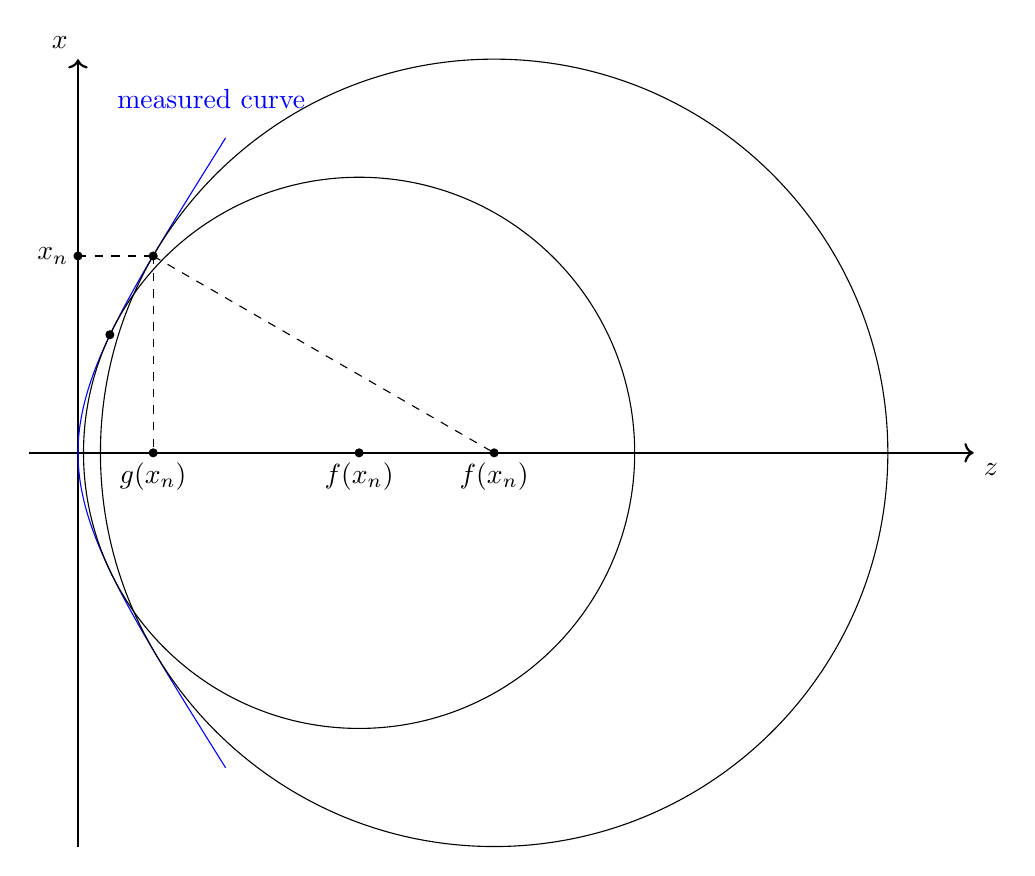
\begin{tikzpicture}
\draw[thick,->] (-1,0) -- (11,0) node[anchor=north west] {$z$};
\draw[thick,->] (-0.375,-5) -- (-0.375,5) node[anchor=south east] {$x$};

\draw[blue] (1.5, 4) .. controls (-1, 0) .. (1.5, -4);

\node [right, blue] at (0, 4.5) {measured curve};

%Measurement 1
\draw (4.91,0) circle (5);

\draw[fill] (4.91,0) circle [radius=0.05];
\node [below] at (4.91,0) {$f(x_n)$};

\draw[fill] (0.58,2.5) circle [radius=0.05];

\draw[fill] (0.58,0) circle [radius=0.05];
\node [below] at (0.58,0) {$g(x_n)$};

\draw[fill] (-0.375, 2.5) circle [radius=0.05];
\node [left] at (-0.375, 2.5) {$x_n$};

\draw[dashed] (-0.375,2.5) -- (0.58,2.5);

\draw[dashed] (0.58,2.5) -- (0.58,0);

\draw[dashed] (0.58,2.5) -- (4.91,0);

%Measurement 2
\draw (3.195,0) circle (3.5);

\draw[fill] (3.195,0) circle [radius=0.05];
\node [below] at (3.195,0) {$f(x_n)$};

\draw[fill] (0.03,1.5) circle [radius=0.05];

\end{tikzpicture}


\end{document}